\documentclass[UTF8,zihao=-4]{ctexart}
\usepackage[a4paper,top=2.4cm,bottom=2.4cm,left=2.5cm,right=2.5cm]{geometry}
\usepackage{amsmath,amssymb}
\usepackage{booktabs}
\usepackage{graphicx}
\usepackage{multirow}
\usepackage{array}
\usepackage{caption}
\usepackage{hyperref}
\usepackage{xcolor}
\usepackage{url}

\graphicspath{{figures/}}
\hypersetup{
  colorlinks=true,
  linkcolor=black,
  citecolor=blue!55!black,
  urlcolor=blue!55!black
}
\captionsetup{font=small,labelfont=bf}
\setlength{\parindent}{2em}
\setlength{\parskip}{0.15em}
\renewcommand{\arraystretch}{1.16}

\title{\textbf{面向图像条件软传感器退化的可靠多模态垃圾分类方法}}
\author{}
\date{}

\begin{document}
\maketitle

\section*{摘要}
多模态垃圾分类能够从视觉外观、类别语义和结构化属性中获得互补信息，但附加观测
一旦缺失或失真，无条件融合反而会放大错误证据。本文提出一种面向图像条件软传感器
退化的可靠多模态分类方法。该方法以YOLO11多尺度视觉表示和CLIP类别文本原型构建
语义上下文，并从视觉--文本联合表示预测可回退的传感器潜表示；样本级门控进一步
结合观测可用性、网格质量、跨模态一致性和异方差不确定性，在观测退化时抑制残差，
在观测缺失时退回预测表示。在由5990张真实采集源图构成、包含19类和8654个对象
记录的内部基准上，三次独立训练的平均Accuracy和Macro F1分别为
$88.26\%\pm0.21$和
$82.26\%\pm0.31$。与匹配训练的无可靠性模型相比，两项指标平均提高0.81和
0.51个百分点，且三次训练的变化方向一致。门控路径干预以及missing、noise、
bias、stuck和mixed退化实验呈现出与设计一致的抑制和回退行为。潜空间方差能够
较好地排序表示误差，但绝对尺度仍偏保守。原始RGB与对象标注来自真实采集图像；
软传感器网格是在这些真实样本上逐条派生的图像条件观测，而非同步物理测量，
当前结论限于内部对象基准和所定义的软件退化条件。

\noindent\textbf{关键词：}垃圾分类；多模态融合；软传感器；模态退化；可靠性门控；
不确定性

\section{引言}

垃圾识别已由封闭集对象分类逐步扩展到自然场景检测、工业传送带分割和自动分选。
WasteNet展示了边缘端视觉分类在智能垃圾桶中的可行路径\cite{white2020wastenet}；
TACO以多边形标注刻画自然环境中的散落垃圾\cite{proenca2020taco}，ZeroWaste则
把研究推进到工业场景中密集、遮挡和可变形目标的实例分割
\cite{bashkirova2022zerowaste}。近期SortWaste和ScatSpotter进一步提示，目标
尺度、拥挤度、伪装外观以及独立采集测试集都会改变识别结果的解释边界
\cite{inacio2026sortwaste,crall2026scatspotter}。这些工作反映出垃圾类别外观
相似、背景复杂和样本分布长尾等困难，也说明对象分类、整图检测与实例分割应当
分别定义任务和指标。

除RGB外观外，材料响应和空间分布能够提供补充线索。已有垃圾分选研究融合RGB、
近红外高光谱、热成像和太赫兹等同步观测\cite{bihler2023multisensor}，
SpectralWaste还在真实分拣设施中建立了同步RGB与高光谱数据
\cite{casao2024spectralwaste}。这类独立物理模态具有明确的传感来源。本文的RGB
与对象标注同样来自真实采集垃圾图像；附加结构化属性则在每个真实对象裁剪上逐条
估计，由视觉语言模型或确定性规则形成一张$4\times4$网格。因此，本文的数据基础
是真实对象样本，网格是与样本一一绑定的派生软观测。该网格用于研究融合、缺失回退
和软件退化机制，但不等同于同步硬件测量。若忽略这一来源层次，平均分类精度很容易
掩盖附加模态何时有效、何时失真以及模型是否真正抑制了错误证据。

一般多模态研究已经证明，融合结构不会天然抵抗模态缺失
\cite{ma2022missing}。现有工作分别从低质量输入的动态融合
\cite{zhang2023quality}、缺失模态的分布一致恢复\cite{wang2023dicmor}、
单模态偶然不确定性\cite{gao2024aleatoric}、概率式缺失模态映射
\cite{chen2024pcd}和超模态增强\cite{zhuang2025hme}等角度提升鲁棒性。然而，
面向图像条件软传感器的垃圾分类仍存在三个相互关联的问题：其一，观测网格与RGB
共享信息来源，质量判断必须区分“有信息”与“独立物理证据”；其二，$4\times4$
空间网格的异常既表现在潜表示差异，也表现在局部统计和跨模态形状不一致；其三，
仅报告最终Accuracy不足以证明可靠性门控确实响应了缺失或退化。

围绕这些问题，本文构建视觉、类别文本与图像条件软传感器的统一对象级分类框架。
视觉--文本上下文预测可回退的传感器潜表示及其异方差，观测网格与预测clean网格
之间的差异则与可用性、原始网格统计和潜空间一致性共同决定门控强度。有效传感器
表示由预测表示和观测残差连续插值得到，使正常利用、退化抑制与完全缺失回退具有
统一的数学形式。后续实验从任务性能、匹配消融、门控行为和退化响应四个角度检验
这一设计。

本文的主要贡献如下。
\begin{enumerate}
  \item 提出一种面向图像条件$4\times4$软传感器退化的可靠多模态垃圾分类结构，
  将视觉--文本条件潜表示预测、观测回退和跨模态质量判别纳入同一前向过程。
  \item 构建由可用性、原始网格质量、跨模态网格差异、潜表示一致性和异方差
  不确定性共同驱动的样本级门控，并通过clean网格重建、可靠性校准和排序目标学习
  退化程度。
  \item 通过匹配重训消融、门控路径干预、五类单项及混合软件退化和潜空间
  不确定性分析，说明该方法在内部基准上的性能变化、作用方式及适用范围。
\end{enumerate}
本文研究对象是19类内部对象基准上的图像条件sidecar；其结论不等同于同步硬件
观测或外部盲测性能。

\section{相关工作}

\subsection{垃圾分类与场景理解}

早期垃圾识别通常把单个对象裁剪输入卷积网络，并以总体分类精度衡量系统性能。
这种设置便于嵌入式实现，但难以覆盖开放环境中的遮挡、密集目标和背景变化。
TACO、ZeroWaste、SortWaste和ScatSpotter分别从野外垃圾、工业传送带、密集
分选和独立采集场景扩展了检测或分割任务
\cite{proenca2020taco,bashkirova2022zerowaste,inacio2026sortwaste,crall2026scatspotter}。
它们共同表明，数据单位、场景分布和评价协议决定了指标能够支持的结论。本文主
任务仍是已知目标框内的19类对象分类，因此采用Accuracy、Macro F1和校准指标；
目标检测和分割只作为系统范围扩展，不能与对象级指标直接比较。

\subsection{垃圾分选中的多模态信息}

垃圾材料常具有相似颜色和形状，独立传感器可从光谱、热响应或太赫兹特征补充
视觉信息。Bihler等融合多类物理传感数据进行大件垃圾分类
\cite{bihler2023multisensor}，SpectralWaste则为同步RGB和高光谱分割提供了
真实设施数据\cite{casao2024spectralwaste}。这些研究的优势来自物理来源的
互补性，同时要求时间同步、空间配准和设备标定。本文侧重另一层问题：当结构化
观测由图像条件估计并可能缺失或退化时，融合模型怎样保留统一接口和可解释回退。
因此，本文不把软传感器带来的变化解释成独立硬件模态增益。

\subsection{低质量与缺失模态学习}

缺失模态鲁棒性大致可分为质量感知融合、表示恢复和不确定性建模三类。动态质量
融合根据输入状态改变模态权重\cite{zhang2023quality}；分布一致恢复和概率蒸馏
利用可用模态补全缺失表示\cite{wang2023dicmor,chen2024pcd}；偶然不确定性方法
则尝试从噪声水平调节模态贡献\cite{gao2024aleatoric}。这些路线为本文提供了
方法依据。在本文检索覆盖的代表性工作中，尚未形成同时面向图像条件
$4\times4$网格空间质量、视觉--文本预测网格一致性和门控路径干预的
统一评价。本文的
差异不在于单独使用注意力、FiLM或异方差，而在于围绕该软传感器来源组织回退、
质量证据和评价闭环。

\section{数据与方法}

整体流程如图\ref{fig:method}所示。RGB目标裁剪和全部类别文本原型先形成视觉--
文本上下文；该上下文预测传感器潜表示与clean网格。观测网格经编码后不直接并入
分类器，而是由可用性、原始网格统计、预测--观测差异及潜空间不确定性共同控制
其相对预测表示的残差。以下依次说明数据治理、三路表示、回退门控和训练目标。

\begin{figure}[htbp]
\centering
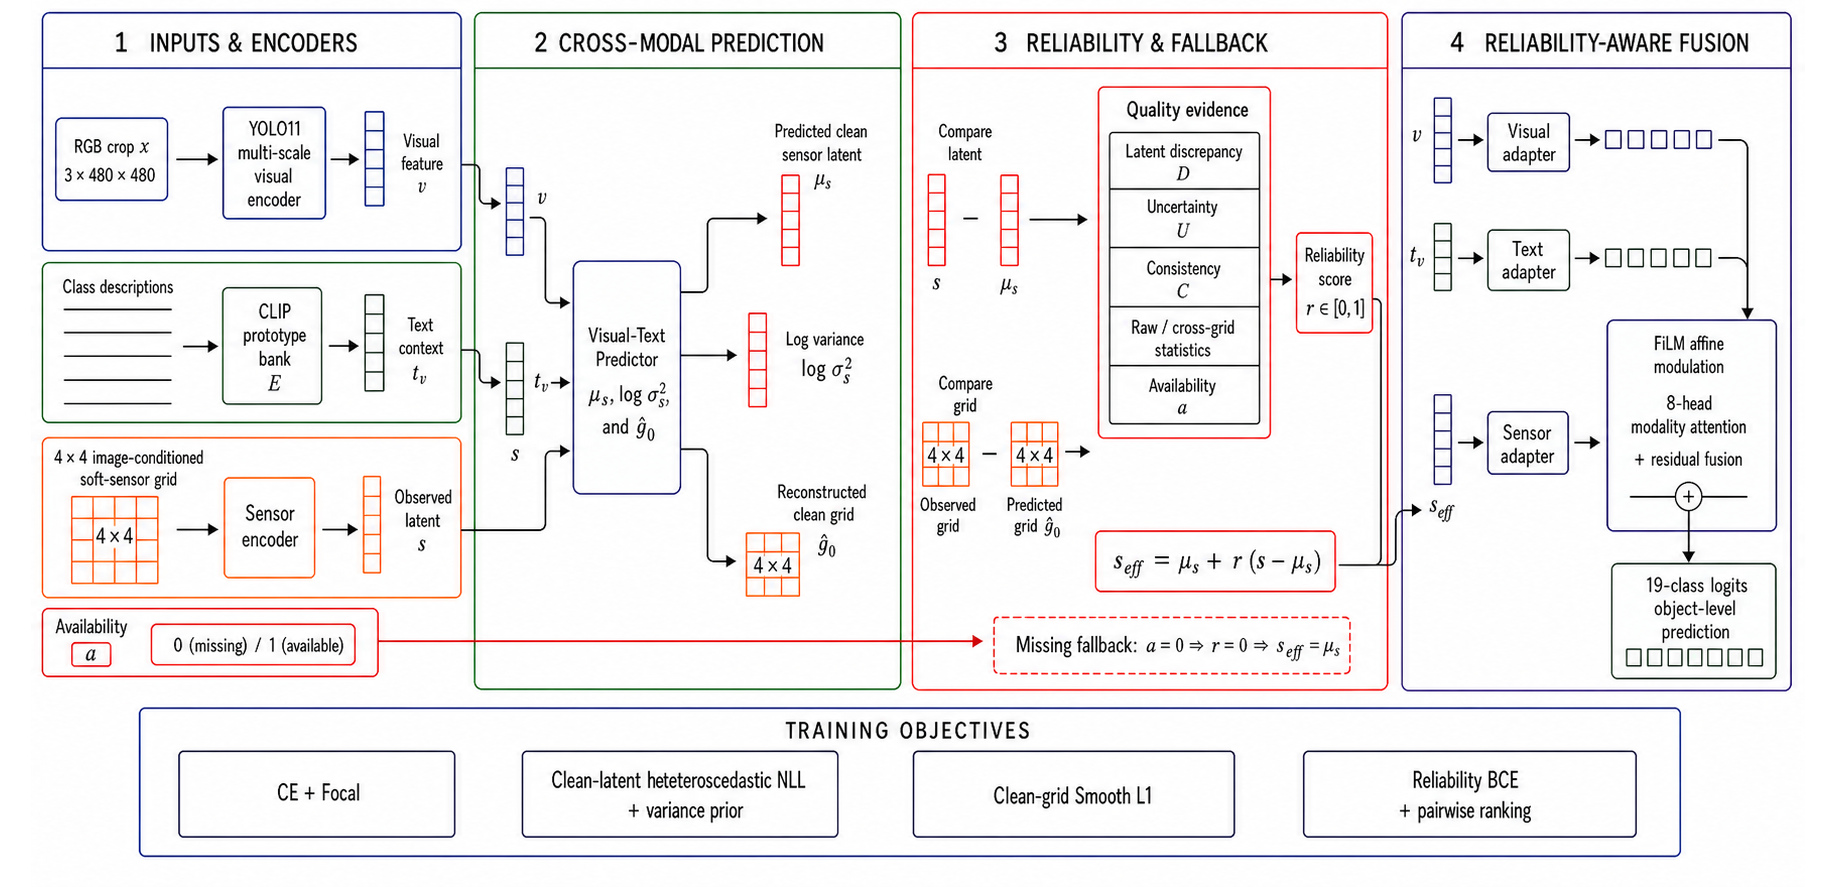
\includegraphics[width=0.98\linewidth]{method_architecture_ai_no_icons_word.jpg}
\caption{跨模态一致性感知的可靠多模态垃圾分类框架。RGB目标裁剪、类别文本原型
和$4\times4$图像条件软传感器分别编码；视觉--文本上下文预测传感器潜表示和
clean网格，多类质量证据估计可靠性，缺失时有效传感器表示回退到预测潜表示。
图中网格来自Qwen/rule图像条件sidecar，不是同步硬件测量。}
\label{fig:method}
\end{figure}

\subsection{任务定义与数据治理}

给定RGB目标裁剪$x$、19个类别文本描述构成的原型集合$E$、可选软传感器网格
$g\in\mathbb{R}^{4\times4}$及其可用性$a\in\{0,1\}$，模型输出类别
$y\in\{1,\ldots,19\}$。对象级主模型不预测边界框或掩码。类别名称沿用原始标注
本体，包含厨余、容器、电池、建材、陶瓷和药品包装等对象，但并非法律或行业标准
意义上的垃圾大类，也不等同于医疗废物类别体系。

原始视觉数据由真实采集的垃圾图像及对象标注组成，共包含8654条对象记录和
5990张源图。划分以哈希化
\texttt{source\_image\_id}为分组单位，同一源图中的对象只进入训练、验证或测试
之一。表\ref{tab:data}给出数据组成。测试集826条对象来自570张源图，后续区间
估计据此按源图聚类。

\begin{table}[htbp]
\centering
\caption{真实图像对象基准的数据划分与软传感器来源。}
\label{tab:data}
\small
\begin{tabular}{lrrrr}
\toprule
集合 & 对象数 & 源图数 & Qwen辅助 & rule-v1回退 \\
\midrule
训练集 & 7002 & 4823 & 6989 & 13 \\
验证集 & 826  & 597  & 826  & 0 \\
测试集 & 826  & 570  & 824  & 2 \\
\midrule
合计   & 8654 & 5990 & 8639 & 15 \\
\bottomrule
\end{tabular}
\end{table}

去重分析识别出8组完全相同的对象裁剪；移除测试集中的1条重复记录后，主要结论
保持不变。跨集合未发现字节级重复，感知哈希、灰度误差和相关性联合筛查得到24对
高相似候选，相关敏感性分析同样未改变主要点估计。按源图分组能够避免直接的文件
泄漏，但由于缺少采集批次和物体实例标识，仍无法完全排除弱相关样本。数据分布还
具有明显长尾：训练集最大类与最小类相差29.75倍，测试集最少类别仅含5个样本。
因此，除总体Accuracy外，本文还报告Macro F1、逐类结果和源图簇置信区间。

\subsection{图像条件软传感器}

每条真实对象记录均关联一份sidecar，其中包含重量、温度、湿度、电导率、气味指数和一张
\texttt{normalized\_grid}。当前网络只读取$4\times4$网格，五个标量不参与
分类，并保留为未来硬件接口的字段。网格按目标裁剪的二维位置排列，每个单元是$[0,1]$
范围内的图像条件响应代理，不对应已校准的压力或材料物理量。qwen3.5-flash
接收目标裁剪和不含类别字段的固定提示词，只返回五项数值属性与严格$4\times4$
JSON网格，生成过程中不提供类别、标签或目标索引。Qwen3-VL模型族的
视觉语言能力由技术报告说明\cite{bai2025qwen3vl}。

确定性rule-v1不读取标签：先把裁剪灰度双线性缩至$4\times4$，再结合亮度反值、
目标框面积、纹理和样本哈希种子构造响应，最后在样本内映射到$[0,1]$。Qwen输出
同样接受数值范围和网格形状校验。8654条记录中，8639条采用Qwen辅助估计，
其余15条因结构化输出不满足约束而使用rule-v1回退。

这些网格逐条绑定真实RGB裁剪，本文将其定义为\textbf{真实样本上的图像条件软
传感器观测}。它们作为数据集中实际保存的逐样本记录参与训练与评估，但其数值由
图像推断，不具有经硬件标定的重量、温湿度、电导率或气味物理量含义。实验直接使用
已保存的sidecar，并公开提示词约束、解析schema和rule-v1实现，以避免托管模型
版本变化影响后续复现。

\subsection{视觉与文本表示}

RGB裁剪经过双边滤波、低亮度条件CLAHE、Laplacian锐化、单位仿射变换和
$480\times480$缩放。YOLO11s-seg\cite{ultralytics2024yolo11}的三个尺度特征
$F_k(x)$经全局平均池化和独立线性投影得到512维token，随后由可学习尺度先验
聚合：
\begin{equation}
 z_k=P_k\!\left(\operatorname{GAP}(F_k(x))\right),\qquad
 v=\sum_{k=1}^{3}\operatorname{softmax}(p)_k z_k .
\label{eq:visual}
\end{equation}
尺度先验初始化为$0.3/0.5/0.2$，YOLO前5层保持冻结。

CLIP ViT-B/16文本塔\cite{radford2021clip}一次编码19条类别描述，得到归一化
原型矩阵$E$。模型不向文本分支输入真实标签，而以视觉token查询全部原型：
\begin{equation}
 t_v=\operatorname{softmax}\!\left(
   \frac{\operatorname{cos}(v,E)}{\tau}\right)E,\qquad \tau=0.07 .
\label{eq:text}
\end{equation}
该早期文本上下文既提供类别语义，也作为预测传感器潜表示的条件。

\subsection{潜表示预测与缺失回退}

记未注入退化的sidecar为clean网格$g^0\in[0,1]^{4\times4}$，软件退化和$[0,1]$截断先
产生观测网格$\tilde g$。原始与跨模态质量头直接读取$\tilde g$；传感器编码器再
按样本执行
$\bar g=(\tilde g-\operatorname{mean}(\tilde g))/
\max(\operatorname{std}(\tilde g),10^{-6})$。因此常数卡死网格会得到有限的零
中心表示，其异常仍可由原始网格flatness、可用性和预测--观测差异识别。
$\bar g$双线性上采样到$16\times16$，经$1\times1$卷积、LeakyReLU和全局池化
得到512维观测表示$s$。视觉与文本上下文共同预测潜表示均值$\mu_s$和有界对数
方差：
\begin{equation}
 \mu_s=g_\mu([v,t_v]),\qquad
 \log\sigma_s^2=l_{\min}+(l_{\max}-l_{\min})
 \operatorname{sigmoid}(g_\sigma([v,t_v])) ,
\label{eq:latent}
\end{equation}
其中$l_{\min}=-3$、$l_{\max}=2$。异方差形式借鉴视觉任务中对数据噪声的建模
\cite{kendall2017uncertainty}。模型进一步计算归一化重建差异$D$、平均预测方差
$U$和余弦一致性$C$：
\begin{align}
 D &= \operatorname{mean}\!\left((s-\mu_s)^2
      \exp(-\log\sigma_s^2)\right), \\
 U &= \operatorname{mean}\!\left(\exp(\log\sigma_s^2)\right), \\
 C &= \frac{\operatorname{cos}(s,\mu_s)+1}{2}.
\label{eq:duc}
\end{align}
实现先截断$D$和$U$，再把$\log(1+D)$与$\log(1+U)$送入可靠性头，以避免极端
方差导致数值不稳定。

\subsection{跨模态质量与可靠性门控}

模型从观测网格提取均值、标准差、动态范围、水平梯度、垂直梯度、饱和率和
flatness七项统计。另由$[v,t_v,\mu_s]$解码预测clean网格$\hat g$，将观测网格与
$\operatorname{stopgrad}(\hat g)$组合为22维跨模态质量特征，包括两组网格统计、
MAE、RMSE、最大误差、均值偏差、余弦相似度、梯度差和availability。停止梯度
避免质量头通过改变预测网格投机降低校准目标。

最终可靠性由潜表示证据、原始网格质量和跨模态网格差异三个logit残差共同决定：
\begin{equation}
 r=a\cdot\operatorname{sigmoid}\!\left(
 h_{\mathrm{lat}}([\log(1+D),C,\log(1+U),a])
 +h_{\mathrm{grid}}(q_g)+h_{\mathrm{cross}}(q_{g,\hat g})\right).
\label{eq:gate}
\end{equation}
\begin{equation}
 s_{\mathrm{eff}}=\mu_s+r(s-\mu_s).
\label{eq:fallback}
\end{equation}
式\eqref{eq:gate}是本文方法的核心：当$a=0$时，$r=0$且
$s_{\mathrm{eff}}=\mu_s$，模型完全回退；当观测可用但质量较低时，$r$连续缩小
观测残差；只有可靠性较高时，表示才接近$s$。该设计与低质量模态动态融合和不确定
性调节的研究动机一致\cite{zhang2023quality,gao2024aleatoric}，但$r$只表示
当前软传感器及已定义退化下的相对可用性，不是物理测量置信度。

\subsection{融合与训练目标}

视觉和有效传感器共同查询类别原型，得到最终文本上下文。三个512维模态分别经过
Adapter、LeakyReLU和dropout，再由FiLM-style逐模态仿射参数调制；FiLM原始形式
参见\cite{perez2018film}，但本文的$\gamma/\beta$是全局参数，不是文本动态生成
网络。模态token下投影到128维后执行8头自注意力，并与动态细化的YOLO尺度表示
残差融合。

退化监督只由clean网格与观测网格的差异构造，不使用类别标签。对第$i$个样本，
质量目标为
\begin{equation}
 q_i=a_i\operatorname{clip}\!\left(
 1-\frac{\frac{1}{16}\lVert\tilde g_i-g_i^0\rVert_1}{0.25},0,1\right).
\label{eq:quality}
\end{equation}
记$s_{\mathrm{clean}}=\operatorname{Encoder}(g^0)$，并令
$\ell_i=\operatorname{logit}(\operatorname{clip}(r_i,10^{-6},1-10^{-6}))$。
总目标包含交叉熵、Focal Loss\cite{lin2017focal}及五项辅助目标：
\begin{align}
 \mathcal{L}_{\mathrm{cls}} &=
 \mathcal{L}_{\mathrm{CE}}+\mathcal{L}_{\mathrm{Focal}}, \\
 \mathcal{L}_{\mathrm{rec}} &=
 \operatorname{mean}\!\left[
 \frac{1}{2}\left((\mu_s-\operatorname{stopgrad}(s_{\mathrm{clean}}))^2
 \exp(-\log\sigma_s^2)+\log\sigma_s^2\right)\right], \\
 \mathcal{L}_{\mathrm{cal}} &=
 \frac{\sum_i\omega_i\,\operatorname{BCE}(r_i,q_i)}
 {\sum_i\omega_i},\qquad
 \omega_i=\begin{cases}3,&q_i=1,\\1,&q_i<1,\end{cases} \\
 \mathcal{L}_{\mathrm{var}} &=
 \operatorname{mean}\!\left((\log\sigma_s^2+2)^2\right), \\
 \mathcal{L}_{\mathrm{grid}} &=
 \operatorname{SmoothL1}(\hat g,g^0).
\label{eq:auxloss}
\end{align}
批内排序对集合
$\mathcal{P}=\{(i,j):i<j,\lvert q_i-q_j\rvert\geq0.05\}$，其目标和总损失为
\begin{align}
 \mathcal{L}_{\mathrm{rank}} &=
 \frac{1}{|\mathcal{P}|}\sum_{(i,j)\in\mathcal{P}}
 \operatorname{BCEWithLogits}\!
 \left(\ell_i-\ell_j,\mathbf{1}[q_i>q_j]\right), \\
 \mathcal{L} &= \mathcal{L}_{\mathrm{cls}}
 +w_{\mathrm{rec}}\mathcal{L}_{\mathrm{rec}}
 +w_{\mathrm{cal}}\mathcal{L}_{\mathrm{cal}}
 +w_{\mathrm{var}}\mathcal{L}_{\mathrm{var}}
 +w_{\mathrm{grid}}\mathcal{L}_{\mathrm{grid}}
 +w_{\mathrm{rank}}\mathcal{L}_{\mathrm{rank}} .
\label{eq:loss}
\end{align}
若$\mathcal{P}$为空，排序项置零。正式权重依次为
$w_{\mathrm{rec}}=0.1$、$w_{\mathrm{cal}}=0.3$、$w_{\mathrm{var}}=0.1$、
$w_{\mathrm{grid}}=0.5$和$w_{\mathrm{rank}}=0.05$；分类两项权重均为1，
Focal Loss采用$\alpha=0.25$、$\gamma=2$。clean潜表示和网格目标均在当前
迭代停止梯度，即使本轮观测缺失也保留监督。

训练退化在逐样本标准化之前作用于$g^0$。missing以0.10概率先把整张网格置零并
令$a=0$，该样本不再接受其他退化；其余样本保持$a=1$，依次以0.50概率叠加逐
单元高斯噪声（标准差均匀采样于$[0.02,0.15]$）、以0.25概率叠加随机方向平面
偏移（绝对幅度均匀采样于$[0.075,0.15]$），并以0.15概率把整张网格卡在该样本
左上角单元值。最终统一截断至$[0,1]$，再计算式\eqref{eq:quality}并进入编码器。
验证与clean test关闭随机退化，鲁棒性实验采用固定场景和固定扰动种子。这里的
$a$只表示数据管线能够明确识别的“记录缺失”；noise、bias和stuck均保持$a=1$，
由质量证据学习抑制。

\section{实验设计}

\subsection{实现设置}

实验基于PyTorch 2.6.0实现，并在NVIDIA RTX 4090 24 GB GPU上完成训练。
视觉分支从
\texttt{yolo11s-seg.pt}初始化，文本分支使用
\texttt{openai/clip-vit-base-patch16}；三路Adapter均为512维，dropout为0.3，
分类前为LayerNorm和线性层。训练采用AdamW，batch size为16，初始学习率
$10^{-4}$，weight decay为$10^{-5}$，前5轮线性warmup，随后余弦衰减，共100个
epoch。模型选择仅依据验证集Accuracy，测试集不参与训练或超参数选择。本文报告
随机种子42、43和44的三次独立训练结果，其中种子42作为预先确定的参考运行。

\subsection{比较设计}

主要比较考察完整模型与无可靠性子系统基线。后者移除传感器潜表示预测、
可靠性门控、原始和跨模态网格质量及相关辅助损失，但保持软件退化训练、三模态
编码、注意力融合、数据、优化器和100轮日程一致；三个变体分别与种子42、43、
44匹配。该比较用于衡量复合可靠性子系统在基线充分重新适应后的总体作用；各辅助
组件的影响则通过后续独立消融分析。

为观察门控在已训练模型中的直接作用，本文还在种子42参考模型上保持权重和输入
不变，仅关闭可靠性路径。该干预用于分析预测行为，不作为独立重训消融的替代。
此外，方差先验模型、类别平衡策略和不同sidecar来源用于补充分析。

\begin{table}[htbp]
\centering
\caption{比较模型、训练关系及研究目的。}
\label{tab:models}
\small
\begin{tabular}{llll}
\toprule
名称 & 是否重训 & 与完整模型的关键差异 & 比较目的 \\
\midrule
完整模型 & 是，种子42/43/44 & 潜表示预测、三类质量证据、门控及五项辅助目标 &
总体性能与训练稳定性 \\
无可靠性基线 & 是，种子42/43/44 & 联合移除完整可靠性子系统，其余训练日程匹配 &
复合可靠性作用 \\
门控路径干预 & 否，仅种子42 & 保持权重不变并关闭已学习可靠性路径 &
门控行为分析 \\
方差先验基线 & 是，仅种子42 & 无预测clean网格及跨模态网格差异 &
方法演进比较 \\
\bottomrule
\end{tabular}
\end{table}

\subsection{指标与统计}

分类指标包括Accuracy、Macro Precision、Macro Recall、Macro F1、Weighted F1、
Top-3 Accuracy、负对数似然、多类Brier score和15箱ECE；ECE的使用背景参见
\cite{guo2017calibration}。ECE直接使用未做温度缩放的softmax最大概率，在
$[0,1]$上按15个等宽箱计算，空箱跳过。单模型区间按570个源图簇执行2000次
百分位bootstrap。
模型差值按相同源图簇执行5000次配对bootstrap，候选与参考共享每次重采样的簇。
精确McNemar检验只作为826个对象正确/错误不对称的敏感性统计，不校正同图多对象
相关性。历史多消融比较对McNemar的$p$值采用Holm校正，主要解释仍以源图簇区间
和训练种子方向为准。

\subsection{软件退化协议}

退化鲁棒性以种子42的参考模型为例，考察clean、完全缺失
\texttt{missing\_100}、标准差0.15的\texttt{noise\_015}、强度0.08的
\texttt{bias\_008}、卡死值\texttt{stuck}和混合退化\texttt{mixed}。每种随机
退化生成5组实例，用于描述同一训练模型对注入变化的敏感性；这些重复不代表独立
训练。主要退化条件与训练时的故障族一致，训练范围外强度、未见故障类型和
availability误报则在第\ref{sec:component-analysis}节单独分析。

\section{结果与讨论}

\subsection{内部测试表现与训练稳定性}

表\ref{tab:seeds}给出完整模型的三次独立训练结果。平均Accuracy为
$88.26\%\pm0.21$，Macro F1为$82.26\%\pm0.31$，三次训练之间的波动较小。
种子42参考模型取得88.14\% Accuracy、82.44\% Macro F1和2.46\% ECE；
按源图聚类得到的Accuracy与Macro F1 95\%区间分别为
$[85.33\%,90.79\%]$和$[76.46\%,86.22\%]$。

\begin{table}[htbp]
\centering
\caption{完整模型在三个训练种子上的内部测试结果。}
\label{tab:seeds}
\small
\begin{tabular}{lrrrrr}
\toprule
训练种子 & Accuracy & Macro P & Macro R & Macro F1 & ECE \\
\midrule
42 & 88.14\% & 81.60\% & 84.89\% & 82.44\% & 2.46\% \\
43 & 88.50\% & 81.38\% & 85.07\% & 82.45\% & 2.87\% \\
44 & 88.14\% & 81.14\% & 84.48\% & 81.90\% & 2.96\% \\
\midrule
均值$\pm$样本标准差 & $88.26\pm0.21$ & $81.37\pm0.23$ &
$84.81\pm0.30$ & $82.26\pm0.31$ & $2.76\pm0.27$ \\
\bottomrule
\end{tabular}
\end{table}

Accuracy与Macro F1之间约6个百分点的差距与类别长尾一致。最少类别在测试集中
只有5条记录，个别错误即可显著改变该类F1。因此，表\ref{tab:seeds}反映的是
内部总体表现和训练稳定性，而非所有少数类别都获得了稳定改善。

\subsection{可靠性机制的匹配消融}

表\ref{tab:matched}给出完整模型相对匹配无可靠性基线的差值。三个训练种子上的
Accuracy和Macro F1均为正，平均差值分别为+0.81和+0.51个百分点。该方向一致性
表明可靠性子系统在基线重新训练适应后仍带来温和收益。与此同时，种子42和43的
Accuracy区间以及三个种子的Macro F1区间均跨越零，说明该收益的幅度仍受训练
随机性和有限样本规模影响。

\begin{table}[htbp]
\centering
\caption{完整模型相对匹配无可靠性重训基线的对象级差值。差值为完整模型减参考；
区间采用5000次配对源图簇bootstrap。}
\label{tab:matched}
\small
\begin{tabular}{lccc}
\toprule
训练种子 & Accuracy差值/百分点（95\%区间） &
Macro F1差值/百分点（95\%区间） & McNemar $p$ \\
\midrule
42 & $+0.36\;[-0.94,+1.68]$ & $+0.53\;[-1.51,+3.00]$ & 0.7201 \\
43 & $+0.73\;[-0.58,+2.13]$ & $+0.27\;[-2.49,+3.32]$ & 0.3616 \\
44 & $+1.33\;[+0.12,+2.62]$ & $+0.73\;[-1.01,+2.61]$ & 0.0614 \\
\midrule
均值$\pm$样本标准差 & $+0.81\pm0.49$ & $+0.51\pm0.23$ & -- \\
\bottomrule
\end{tabular}
\end{table}

门控路径干预进一步揭示了已训练模型对可靠性分支的依赖。在种子42参考模型中，
保留门控相对关闭门控使Accuracy和Macro F1分别提高2.78和3.50个百分点，
对应95\%区间为$[1.23,4.33]$和$[1.46,5.89]$，精确McNemar
$p=0.0001911$。这一差异大于独立重训的平均效应，可能是因为无可靠性基线能够
在训练中形成替代路径，而直接关闭门控会扰动完整模型已经形成的表示分配。因此，
该结果说明门控确实参与了预测过程，但不构成独立于重训消融的因果证明。

\subsection{软件退化下的抑制与回退}

表\ref{tab:degradation}和图\ref{fig:robustness}比较参考模型在六个观测条件下
的表现。完整模型在missing、noise、bias、stuck和mixed中的Accuracy与Macro F1
差值均为正，其中完全缺失和强噪声的Macro F1差值分别为+2.04和+2.12个百分点。
这与式\eqref{eq:gate}的预期一致：缺失时模型完全使用预测潜表示，网格偏移或
卡死时则由质量证据缩小观测残差。

\begin{table}[htbp]
\centering
\caption{参考模型在软件退化下相对匹配无可靠性基线的效应。ECE改善为正表示
完整模型的ECE更低。}
\label{tab:degradation}
\small
\begin{tabular}{lrrr}
\toprule
场景 & Accuracy效应/百分点 & Macro F1效应/百分点 & ECE改善/百分点 \\
\midrule
clean        & +0.36 & +0.53 & +0.08 \\
missing\_100 & +0.97 & +2.04 & +0.74 \\
noise\_015   & +1.38 & +2.12 & -0.06 \\
bias\_008    & +0.80 & +1.35 & -0.03 \\
stuck        & +0.85 & +0.91 & +0.47 \\
mixed        & +0.73 & +0.93 & +0.42 \\
\bottomrule
\end{tabular}
\end{table}

\begin{figure}[htbp]
\centering
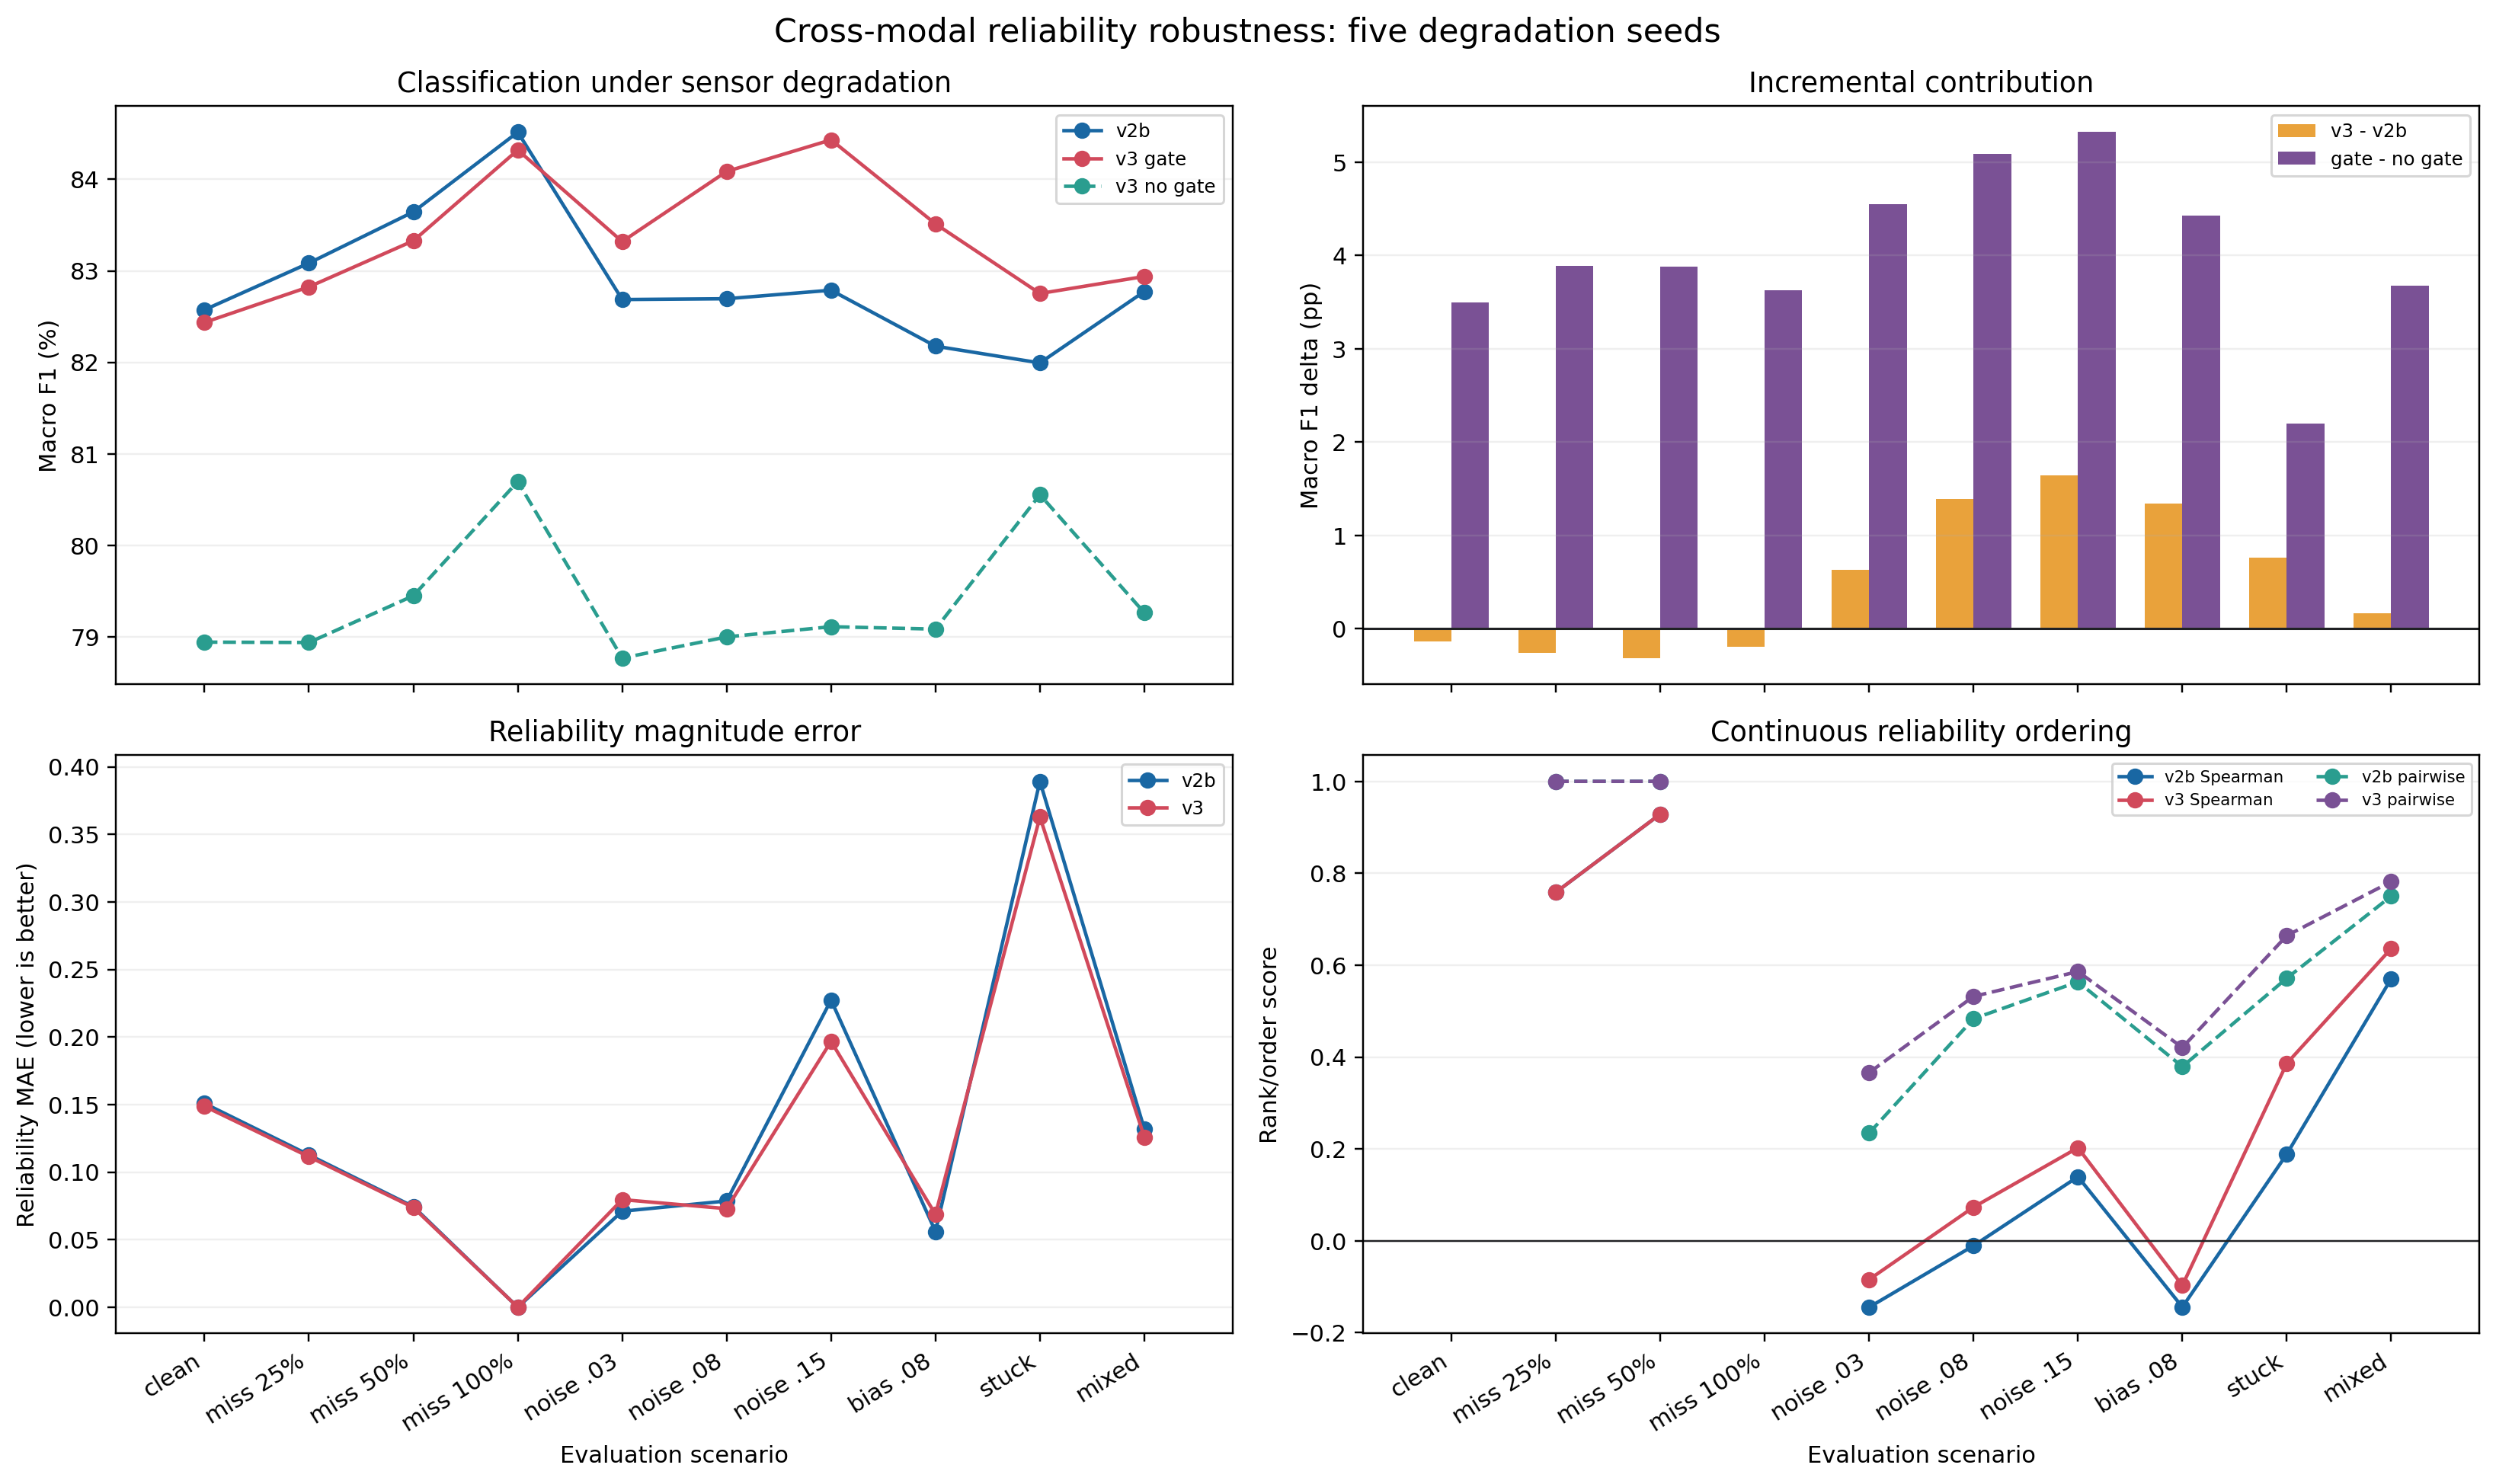
\includegraphics[width=0.98\linewidth]{robustness_comparison.png}
\caption{方差先验基线、完整模型及门控关闭版本（图中分别记为v2b、v3和
v3 no gate）在clean、missing、noise、bias、stuck和mixed条件下的分类与
可靠性表现。每种随机退化由五组软件注入实例汇总。}
\label{fig:robustness}
\end{figure}

校准指标与分类性能并未始终同步变化。noise和bias条件下的ECE分别增加0.06和
0.03个百分点，表明门控改善了分类结果，却尚未在所有退化类型上形成一致的置信度
校准。由于该组实验采用单个参考训练，其作用主要是解释模型的退化响应；总体效应
仍以表\ref{tab:matched}的三次匹配训练为依据。

% BEGIN AUTO PLAN_A_CONFIRMATORY
% Auto-generated from frozen Plan A confirmatory outcomes.
\subsection{组件分析、分布外退化与方法比较}
\label{sec:component-analysis}

为分析辅助目标的作用，本文分别移除网格重建监督和可靠性排序监督，并保持其余
数据、模型和训练设置一致。表\ref{tab:plan-a-components}显示，移除两项监督后
Accuracy和Macro F1均出现约0.5--0.6个百分点的平均下降。

\begin{table}[htbp]
\centering
\caption{移除辅助监督后的三次独立训练结果（均值$\pm$样本标准差）。}
\label{tab:plan-a-components}
\small
\begin{tabular}{lrrrr}
\toprule
变体 & Accuracy & Macro F1 & $\Delta$Acc (pp) & $\Delta$F1 (pp) \\
\midrule
无网格重建监督 & 87.73$\pm$0.30 & 81.63$\pm$0.60 & +0.52$\pm$0.18 & +0.63$\pm$0.42 \\
无可靠性排序监督 & 87.73$\pm$0.60 & 81.65$\pm$0.76 & +0.52$\pm$0.81 & +0.61$\pm$0.88 \\
\bottomrule
\end{tabular}
\end{table}

网格重建监督在三次训练的Accuracy和Macro F1上均呈正向作用；可靠性排序监督在
Macro F1上同样保持一致方向，而Accuracy在其中一次训练中未提高。该结果支持两项
辅助目标的互补作用，但效应幅度仍然有限。

在训练故障族之外，本文进一步考察范围外强度、脉冲、非线性、空间置换、异物替换、
中值卡死和availability误报等11种软件条件。多数条件下，模型性能与clean条件
相近或略高；中值卡死是唯一造成平均Macro F1下降的条件，降幅为0.38个百分点。
这说明模型对多种结构变化具有一定容忍度，但对缺乏区分度的恒定中值观测仍较敏感。

\begin{table}[htbp]
\centering
\caption{完整模型在训练故障族之外的软件条件下的三次训练结果。}
\label{tab:plan-a-unseen}
\scriptsize
\begin{tabular}{lrrr}
\toprule
条件 & Accuracy & Macro F1 & F1相对clean (pp) \\
\midrule
干净观测 & 88.26$\pm$0.21 & 82.26$\pm$0.31 & +0.00 \\
范围外噪声0.30 & 89.06$\pm$0.14 & 83.75$\pm$0.90 & +1.49 \\
范围外偏移0.30 & 88.78$\pm$0.60 & 83.48$\pm$1.18 & +1.22 \\
脉冲故障25\% & 88.74$\pm$0.12 & 83.24$\pm$0.80 & +0.97 \\
非线性响应gamma=2 & 89.02$\pm$0.43 & 83.11$\pm$0.77 & +0.85 \\
空间位置打乱 & 88.86$\pm$0.21 & 83.05$\pm$0.55 & +0.78 \\
异物样本替换 & 88.86$\pm$0.42 & 83.51$\pm$0.65 & +1.25 \\
中值卡死 & 87.93$\pm$0.30 & 81.89$\pm$0.91 & -0.38 \\
正常观测误报缺失 & 88.90$\pm$0.25 & 84.30$\pm$0.03 & +2.03 \\
缺失观测误报可用 & 88.74$\pm$0.12 & 82.85$\pm$0.77 & +0.58 \\
缺失且正确标记 & 88.90$\pm$0.25 & 84.30$\pm$0.03 & +2.03 \\
\bottomrule
\end{tabular}
\end{table}

方法比较选取QMF的质量感知动态决策融合\cite{zhang2023quality}和TMC的
Dirichlet证据组合\cite{han2021trusted}。为控制输入差异，两种方法均复用本文的
视觉编码器、类别文本原型、$4\times4$ sidecar和数据划分，仅替换融合与目标函数。
在这一统一设置下，完整模型的Accuracy和Macro F1均高于两种适配基线。QMF结果
来自三次独立训练；TMC受计算成本限制仅报告一次训练，因此后者只用于提供量级参考。

\begin{table}[htbp]
\centering
\caption{统一输入设置下直接方法基线在clean条件中的结果。}
\label{tab:plan-a-baselines}
\small
\begin{tabular}{lrrrr}
\toprule
方法 & Accuracy & Macro F1 & 相对完整模型Acc (pp) & 相对完整模型F1 (pp) \\
\midrule
QMF适配 & 84.79$\pm$1.10 & 78.37$\pm$0.67 & -3.47 & -3.90 \\
TMC适配 & 80.15 (n=1) & 68.86 (n=1) & -7.99 & -13.58 \\
\bottomrule
\end{tabular}
\end{table}

这些对照反映的是统一输入和内部数据划分下的相对表现，不等同于对原方法完整训练
流程的逐项复现；其中TMC的单次训练结果也不用于讨论训练稳定性。
% END AUTO PLAN_A_CONFIRMATORY

\subsection{潜表示不确定性诊断}

图\ref{fig:uncertainty}在826条测试样本、512维传感器潜空间中比较预测方差和
实际潜表示误差。完整模型的样本均值Spearman相关系数为0.892，说明较高预测方差通常
对应较大潜表示误差；相对方差先验基线（v2b），该相关性增加0.070，源图簇
bootstrap区间为
$[0.0477,0.0954]$。同时，预测方差与实际MSE之比仍为44.3，标准化残差绝对值
小于1.96的覆盖率接近100\%。因此，当前异方差具有较好的相对排序，却在绝对尺度
上明显过分散。

\begin{figure}[htbp]
\centering
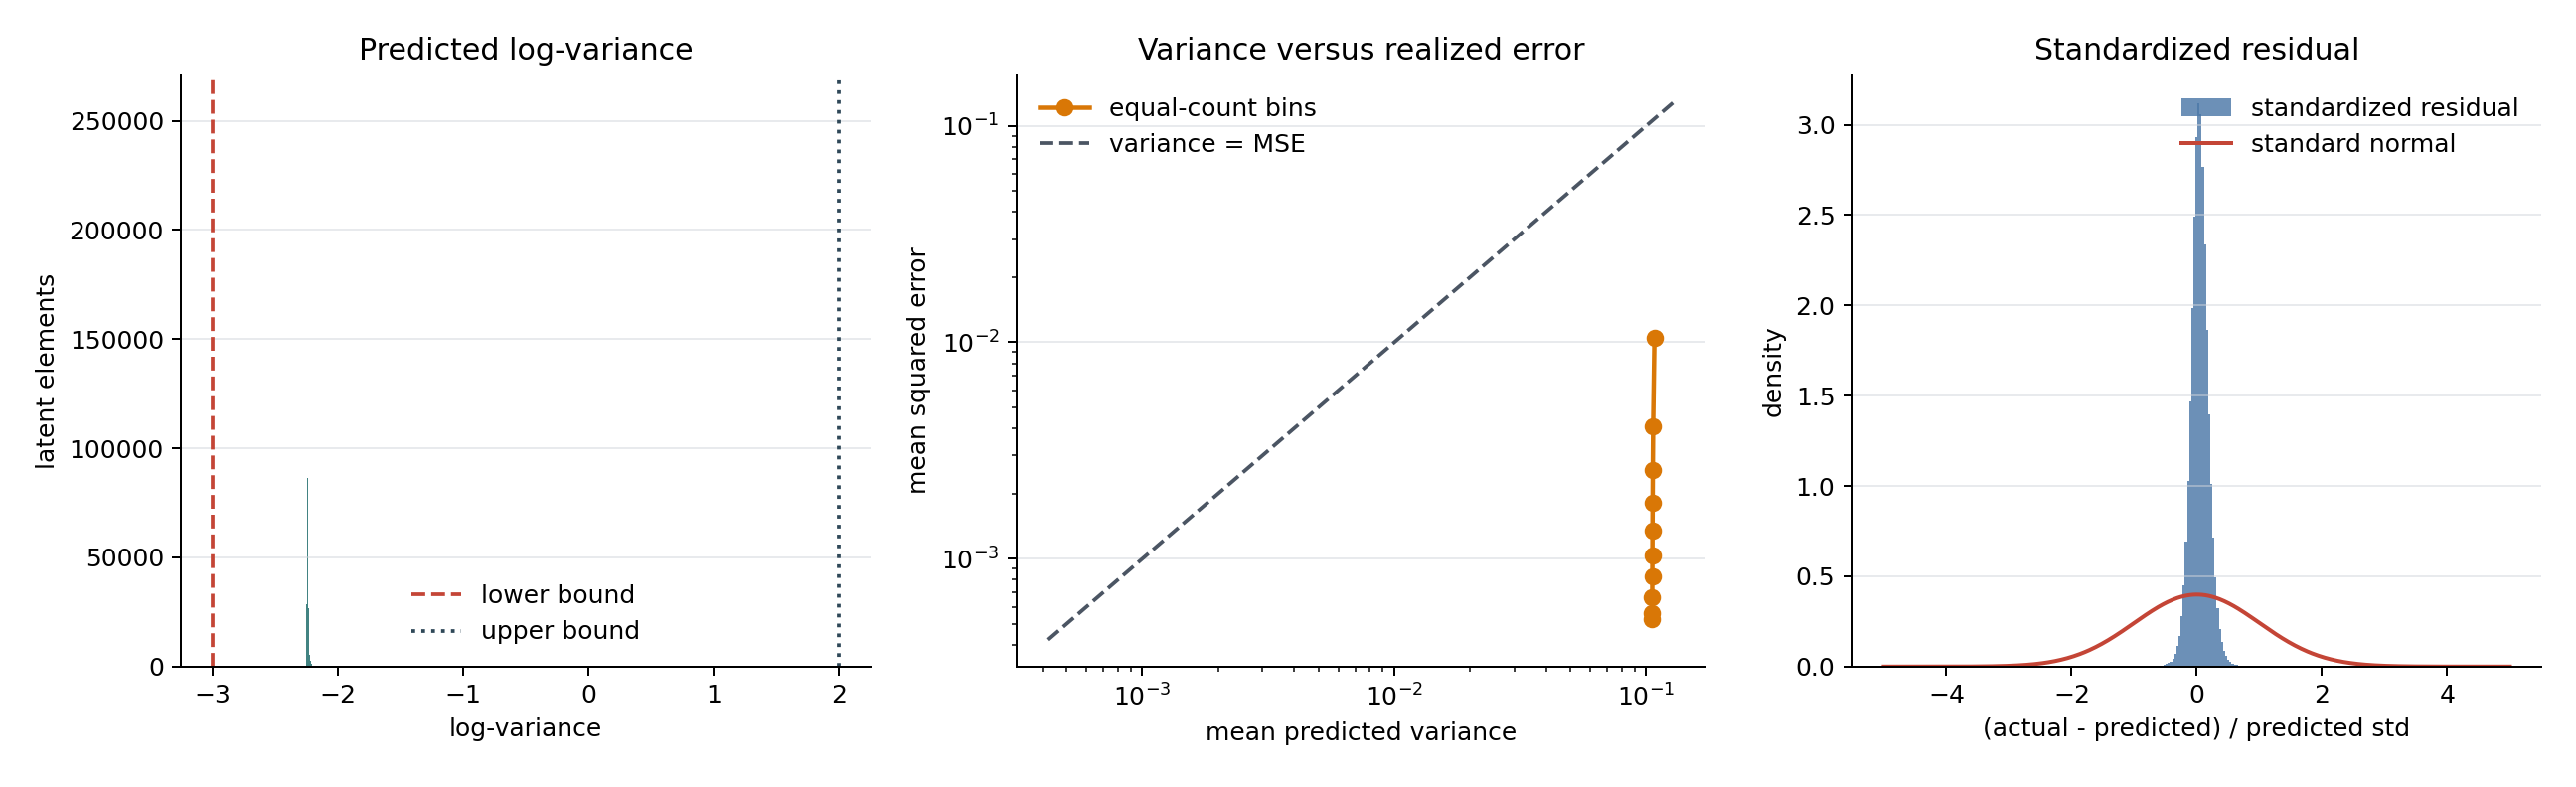
\includegraphics[width=0.98\linewidth]{uncertainty_diagnostics.png}
\caption{完整模型在内部测试样本、512维传感器编码空间上的异方差诊断。左图为
预测对数方差及配置边界，中图比较等频分箱后的预测方差和潜表示均方误差，右图
比较标准化残差与标准正态密度。该诊断不具有物理传感器单位。}
\label{fig:uncertainty}
\end{figure}

这一结果也解释了为何不应只从异方差重建损失的符号判断训练质量。高斯NLL包含
对数方差项，数值可以为负；本文已把下界由早期配置的-6调到-3并增加方差先验，
聚合重建项不再贴近理论下限。然而，方差先验和范围约束只缓解数值塌缩，并未完成
量值校准。当前不确定性更适合作为可靠性排序特征，而不是物理测量误差估计。

\subsection{补充分析与软传感器来源}

早期八项结构消融的Holm校正McNemar检验最小$p$值为0.4767，未显示某一标准融合
组件能够单独解释整体性能变化。类别平衡策略提高了部分少数类Recall，但没有改善
验证集或测试集Macro F1，说明当前误差并不能仅通过重加权解决。图
\ref{fig:class}进一步显示，逐类F1与训练支持量具有明显关联，长尾类别仍是限制
Macro F1的主要因素之一。

\begin{figure}[htbp]
\centering
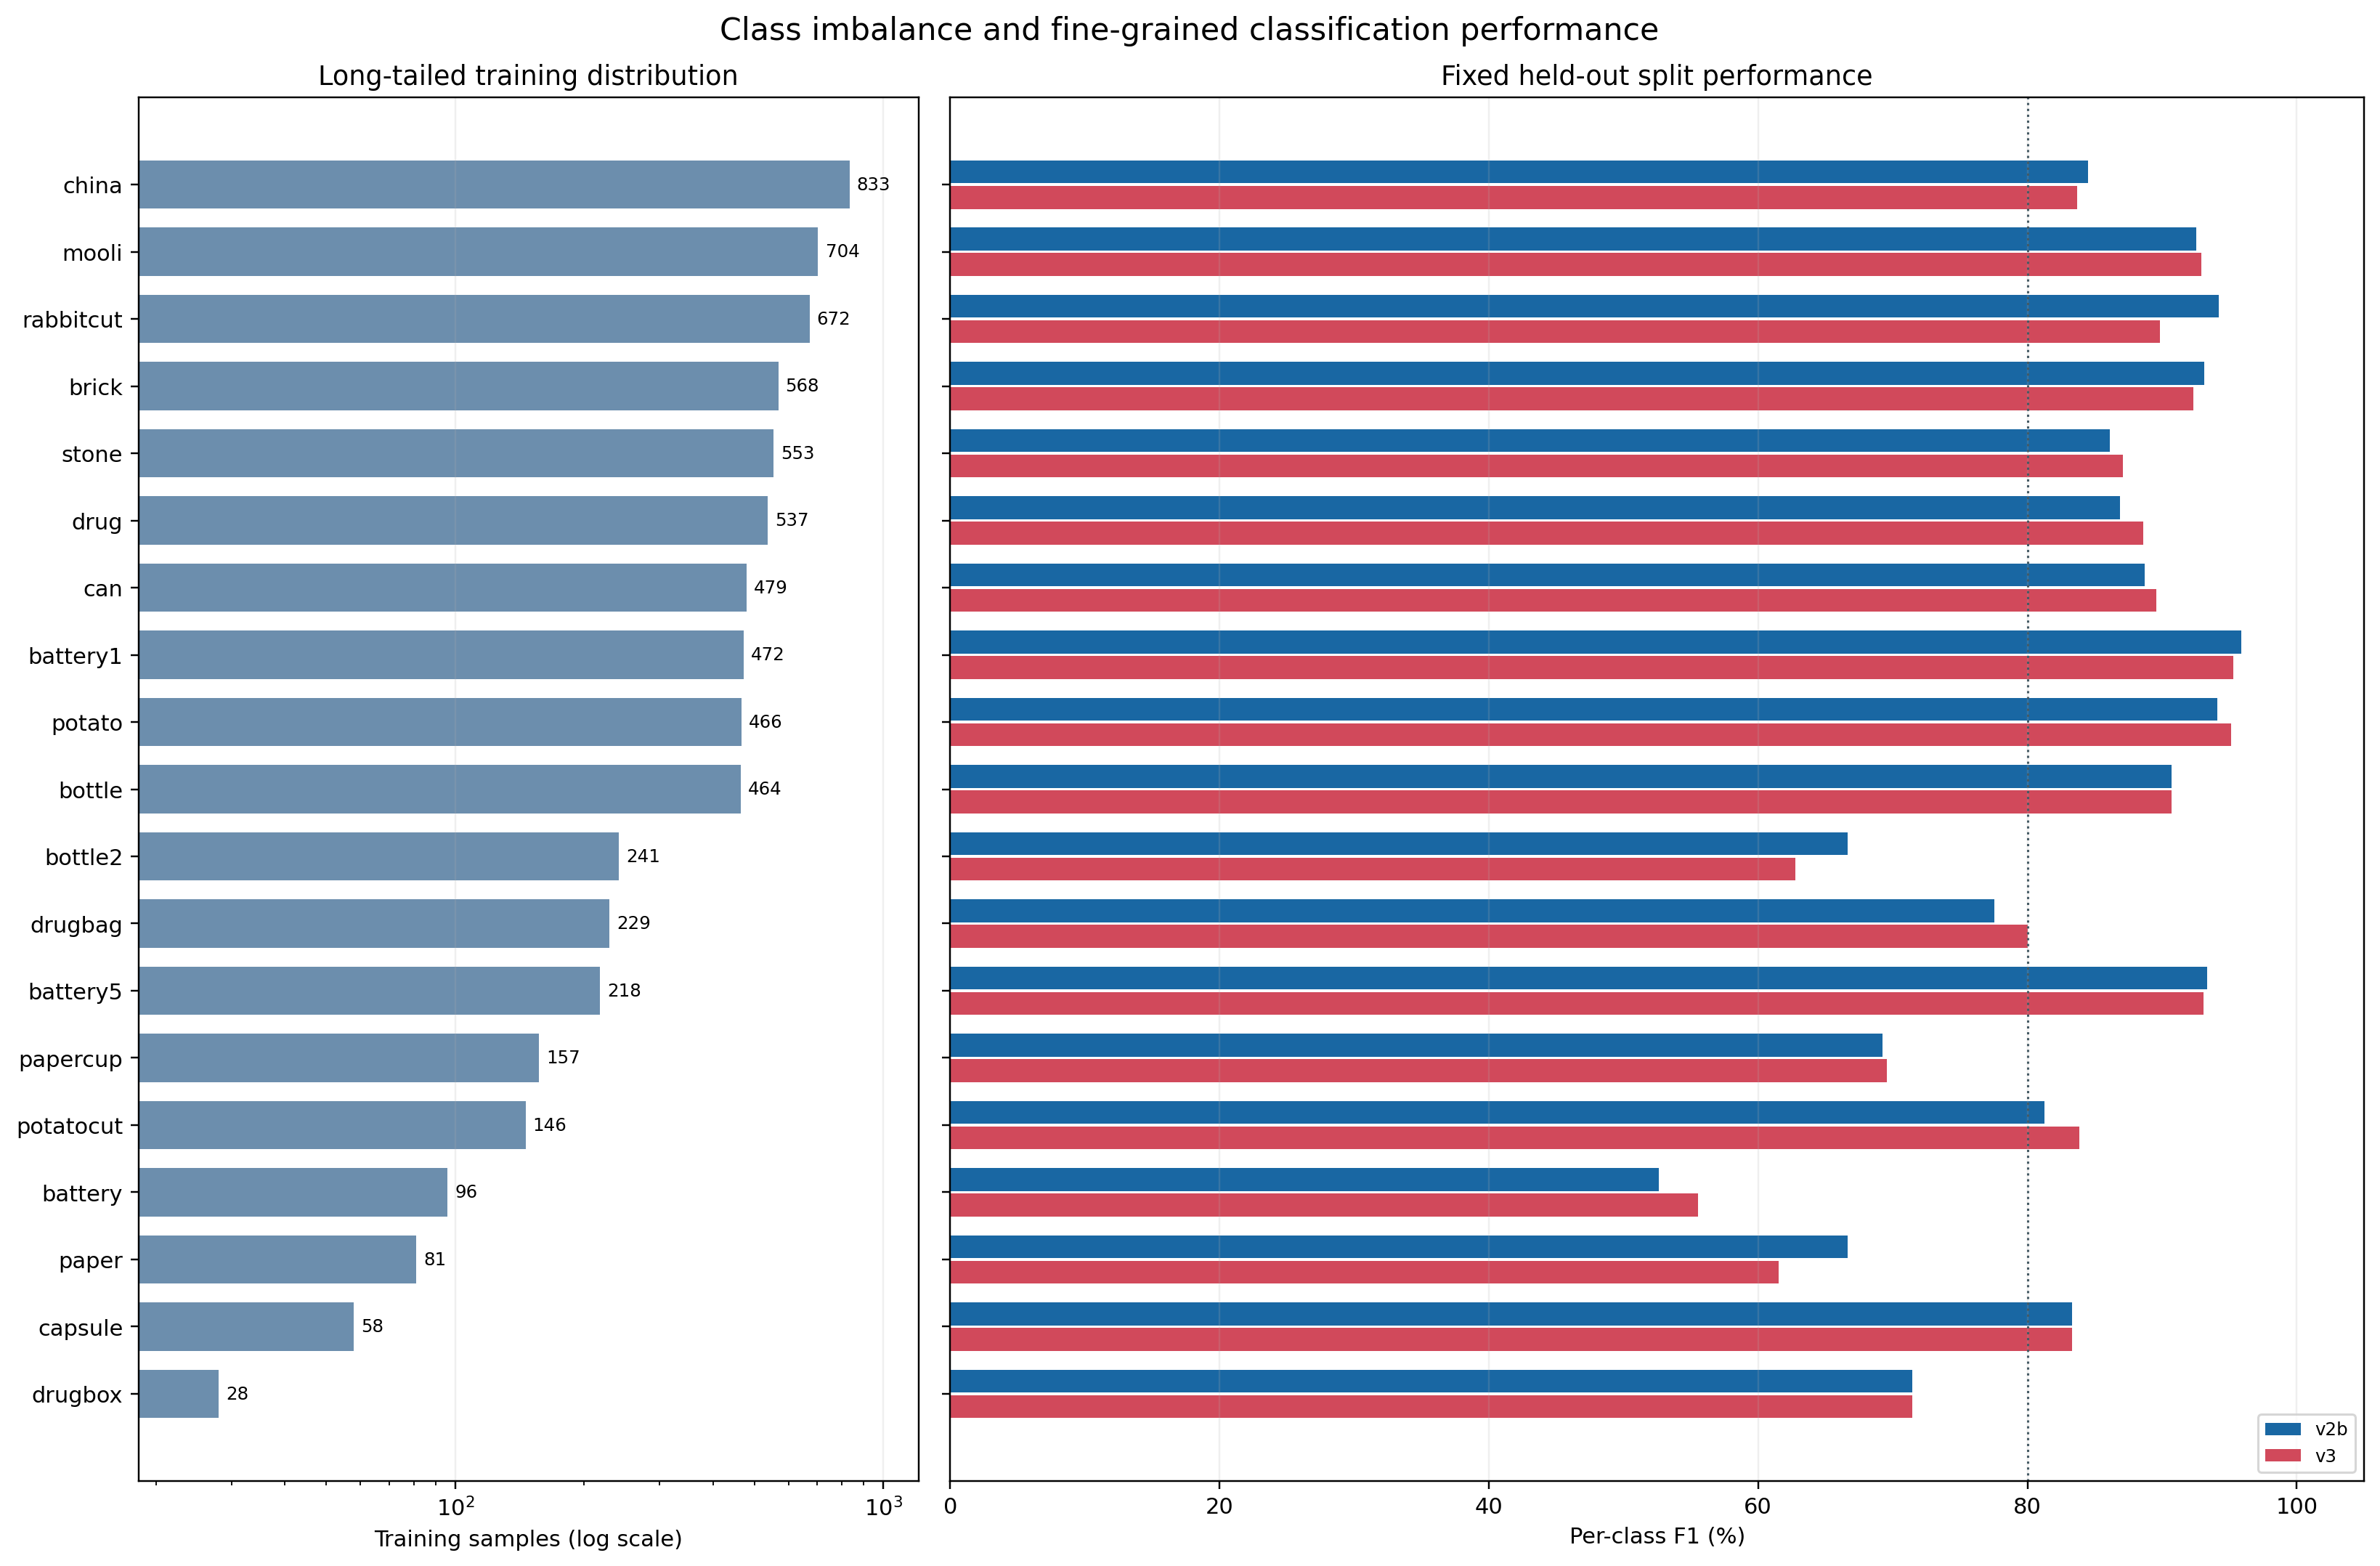
\includegraphics[width=0.92\linewidth]{class_performance_v2b_v3.png}
\caption{方差先验模型（v2b）与完整跨模态质量模型（v3）在826条内部测试记录上
的逐类F1及训练支持量。}
\label{fig:class}
\end{figure}

在真实对象样本的软传感器来源比较中，Qwen sidecar模型的Accuracy/Macro F1为
88.14\%/82.44\%，rule-v1模型为87.29\%/81.87\%。两者的配对区间跨越零，
且都共享RGB图像来源，因此该结果只能说明生成策略存在轻微差异，不能推导出视觉
语言模型或物理传感器的稳定增益。RGB学生对Qwen网格的蒸馏同样未改善分类
Accuracy，表明软目标的拟合质量并不会自然转化为任务收益。

\subsection{系统扩展}

系统扩展方面，独立RGB YOLO11s-seg在570张测试源图、825个唯一对象上取得
box mAP50-95 96.55\%和mask mAP50-95 95.13\%。把文本与RGB预测软传感器
adapter接入原生Segment head后，三个种子的box/mask mAP50-95为
$97.09\%\pm0.02$和$95.34\%\pm0.02$个百分点，变化较小；正式前向仍只读取
RGB。该扩展说明接口能够接入目标域分割头，但不属于对象级可靠性收益，也不是
RGB-D或硬件多模态验证。

\subsection{局限性与外部有效性}

数据层面的限制主要来自内部测试集的重复使用、采集元数据不足和类别长尾。测试集
未参与梯度训练，但已用于多轮研究判断，因此不能视为一次性外部盲测；按源图分组
也无法完全排除同批次或相邻帧相关性。少数类别样本有限，使逐类F1和Macro F1仍
具有较宽的不确定区间。

模态层面的限制更为关键。尽管每个$4\times4$网格都逐条绑定真实RGB对象记录，
其数值仍由图像条件估计，而非与RGB同步采集和标定的物理阵列；所考察的故障也
主要是确定性软件注入，尚不能代表实体
传感器失效或跨设备迁移。QMF和TMC对照复用了本文的数据与编码器，其中TMC仅包含
一次训练，因而方法比较仍需在更充分的统一基准上验证。当前结构虽然与原专利中的
多尺度视觉、文本语义和网格融合思路部分对应，但尚未实现RGB-D输入或硬件阵列，
不构成完整专利系统复现。

\subsection{复现性声明}

训练配置、环境依赖、检查点哈希、sidecar清单、逐样本预测和统计脚本均随实验
归档。所有正式结果均由完整可读检查点生成；训练过程中出现的数据解码和检查点
异常及其恢复方式另行记录，且未涉及验证或测试输入。该归档使主要表格和图件能够
回溯到相应模型与预测文件。

\section{结论}

本文提出了一种面向图像条件软传感器退化的可靠多模态垃圾分类方法。该方法将
视觉--文本条件预测作为传感器表示的回退基础，并利用网格质量、跨模态一致性和
异方差不确定性调节观测残差，从而在统一结构中实现正常利用、退化抑制和完全缺失
回退。内部实验表明，完整模型相对无可靠性基线获得了方向一致但幅度温和的分类
收益；门控路径干预、软件退化和潜空间诊断进一步说明，这些收益与模型对低质量
证据的选择性使用有关。

目前的证据仍限于19类真实图像内部基准及其图像条件sidecar。潜空间不确定性具备
较好的误差排序能力，但绝对尺度尚未校准，软件退化结果也不能替代真实硬件验证。
后续工作将
接入与RGB同步采集的物理阵列，依据采集批次重新划分数据，并在模型与分析方案确定
后开展一次性外部盲测，以检验该方法在跨设备和真实故障条件下的有效性。

\bibliographystyle{unsrt}
\bibliography{references}

\end{document}
